\section{总体风险判断}

总体风险为\textbf{高}。1,024 卡实物展示降低了“产品是否存在”的风险，却没有关闭 8,192 卡规模化、950DT/HiZQ 量产、客户验收、供应商分配、软件有效利用率和公司盈利转化的缺口。对 Atlas 专属供应商归因属于 L4 论点风险；高估值主题篮子的市场风险处于 L3--L4。当前模型的 Atlas 专属收入和 EPS 均为 0，因此路线图延后不会直接削减模型中的 Atlas 利润，却会移除催化剂与倍数期权，价格仍可能大幅回撤。

\begin{exhibitbox}[核心风险矩阵]
\begin{longtable}{L{3.2cm}L{1.3cm}L{1.4cm}L{3.7cm}L{4.0cm}}
\toprule
\textbf{风险} & \textbf{等级} & \textbf{概率} & \textbf{早期指标} & \textbf{估值后果/失效条件}\\
\midrule
\endhead
2026Q4 路线图转交付 & L4 & 45\% & 950DT 可用、客户/站点、验收与收入 & 年底无已验收客户或延至 2027Q1 后，主题倍数压缩 15\%--30\%\\
1,024 到 8,192 卡扩展 & L4 & 55\% & 8,192 卡实物、烧机、通信效率、可用性 & 2027H1 无稳定客户系统，移除全规模架构溢价\\
256TB 内存定义 & L3 & 65\% & 本地/池化层级、带宽、时延 & 若并非本地 HBM，HBM 含量叙事下修 15\%--30\%\\
950DT/HBM/封装良率 & L4 & 50\% & 芯片步进、良率、量产和规格 & 量产延后或降规，系统量与相关期权显著下修\\
UnifiedBus/软件利用率 & L4 & 50\% & 作业完成率、利用率、迁移时间、成本/Token & 生产负载持续不及预期，平台相关倍数压缩 15\%--35\%\\
供应商/BOM/订单分配 & L4 & 80\% & 公司公告、认证、订单、份额和 ASP & 未完成证据链却计入 EPS，构成发布阻断\\
供电/液冷/光学 BOM 未知 & L3 & 70\% & kW/柜、CDU、端口、模块、OCS/UBoE 拓扑 & 外购含量更低或内制，相关主题倍数下修 10\%--30\%\\
客户资本开支与验收 & L4 & 50\% & 客户、站点、电力、付款、利用率与复购 & 无重复部署或利用率低，主题下修 15\%--35\%\\
营运资金与利润率 & L3 & 50\% & 存货/应收天数、经营现金流、分部毛利 & 收入增长但毛利下降超 300bp，EPS 与倍数同时下调\\
客户集中度 & L4 & 40\% & 前五客户、回款和续单 & 拓维等高集中公司发生采购/回款变化，个股下行 20\%--40\%\\
估值拥挤 & L4 & 60\% & 换手、盈利修正、价格/利润背离 & 当前到 Bear 价值的潜在回撤约 10\%--61\%\\
传闻与供应商过度归因 & L4 & 80\% & 监管问答、公司澄清/否认与成交异常 & 否认或长期无公告，传闻溢价可回撤 20\%--40\%\\
\bottomrule
\end{longtable}
\sourcenote{风险矩阵与反方审计。概率为未来 12--18 个月风险预算判断，不是统计预测。}
\end{exhibitbox}

\begin{figure}[htbp]
\centering
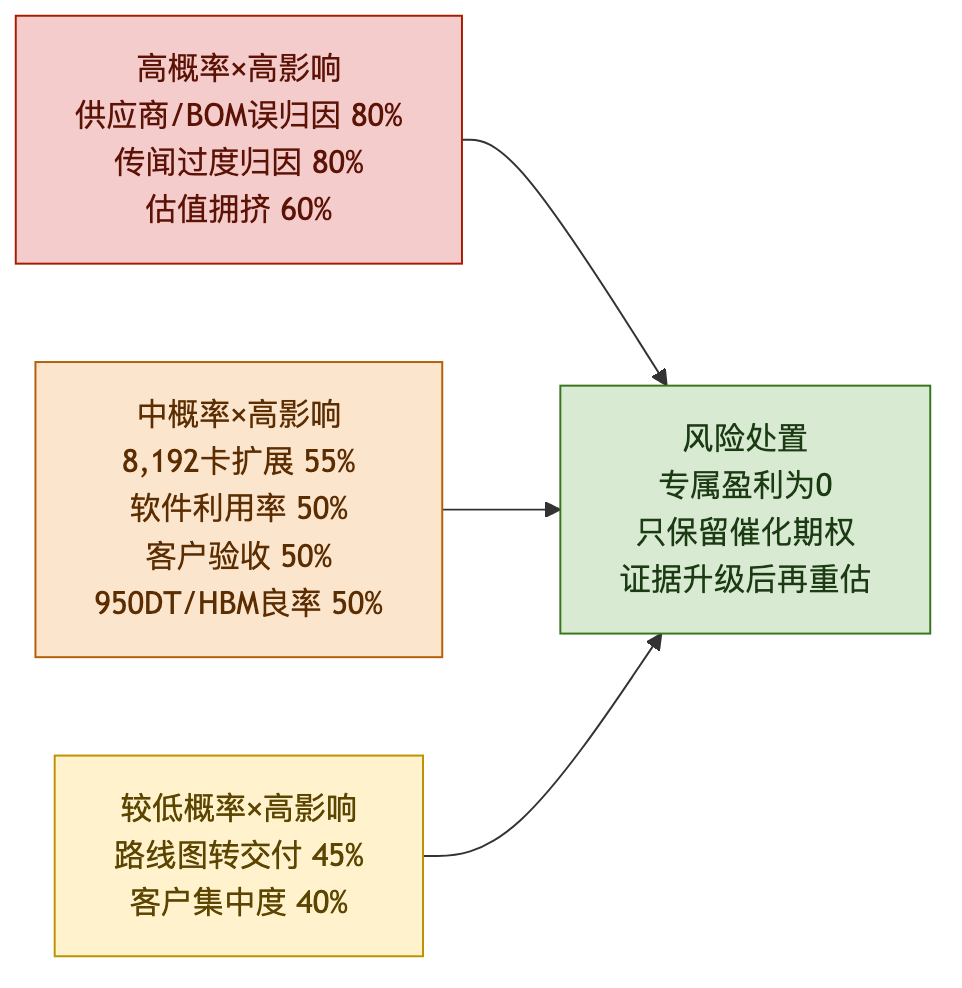
\includegraphics[width=0.96\textwidth]{exhibits/risk_heatmap.png}
\caption{风险概率、影响与模型处置的分层热图}
\sourcenote{核心风险矩阵。概率是未来 12--18 个月风险预算判断；处置以零专属盈利信用和证据升级闸门为核心。}
\end{figure}

最高风险不是系统不存在，而是供应商/BOM 误归因和拥挤定价把技术进展提前转成上市公司利润。中概率高影响组集中在 8,192 卡扩展、软件利用率、客户验收和关键芯片/内存量产；其共同处置不是预测一个精确损失，而是保持 Atlas 专属盈利为 0，只把按期交付作为倍数期权。

\section{地缘政治、合规与 ESG/HRF}

华为仍受美国实体清单和外国直接产品规则约束；高带宽内存、半导体设备和相关软件管制可能同时影响芯片、封装和良率。风险不是“国产替代需求越强就一定越利好”：管制一方面扩大主权算力需求，另一方面可能收紧关键输入、提高成本和延迟量产。2026 年的执法和解案例也说明，涉及华为受控物项的供应链合规风险持续存在。

科大讯飞和部分双用途/国防邻近公司还需结合具体投资授权执行受限实体、人权、数据安全和最终用途审查。报告只能提示风险，不能在不知道用户授权、组合与流动性约束的情况下给出仓位、止损或对冲指令。若授权明确禁止相关实体或用途，估值空间不再重要，应直接排除。

\section{最强反方：系统可以成功，上市公司交易仍可能失败}

最强反方不是“Atlas 950 不存在”，而是“系统真实不等于上市供应商利润拐点”。完整乐观链条为：1,024 卡实物 $\rightarrow$ 950DT/HiZQ 量产 $\rightarrow$ 8,192 卡稳定扩展 $\rightarrow$ UnifiedBus/软件有效利用 $\rightarrow$ 客户采购与验收 $\rightarrow$ 供应商分配 $\rightarrow$ 收入 $\rightarrow$ 毛利 $\rightarrow$ 现金 $\rightarrow$ EPS $\rightarrow$ 估值上行。当前公开证据到达第一节点；科大讯飞提供下游协同，申菱和拓维提供更广义华为/昇腾关系，但没有上游公司完成整条链。

即使华为按时交付，也可能通过内制、多供应商和架构变化压缩外部利润池。UBoE 可能减少交换机和光模块，正交无缆设计可能转移线缆/PCB/连接器价值，华为数字能源或整机集成可能吸收供电/液冷环节。与此同时，项目交付会先占用存货、应收和工程资源，利润与现金可能晚于订单。申菱与英维克 2026Q1 利润承压、拓维扣非亏损，已经提示“关系/订单—利润—现金”并非同步。

\begin{riskbox}[反方证伪协议]
反方被证明错误，需要四层证据同时改善：系统层有客户/站点/验收；工程层有持续负载、可用性、内存层级和故障恢复；供应商层有产品、认证、分配、订单与 ASP；经济层有收入、分部毛利、EPS 和现金流。股价上涨、发布会口号或一般合作不能替代任何一层。
\end{riskbox}

\section{七类压力情景}

第一，路线图延后一个至两个季度，只打击倍数期权；第二，8,192 卡稳定性不足，移除全规模溢价；第三，HBM/封装良率不足，系统量和成本同时恶化；第四，UBoE/CPO/内制降低传统 BOM，系统成功但外部供应商失配；第五，客户站点电力和验收延后，收入与现金后移；第六，收入兑现但毛利率下降、应收存货扩张，EPS 低于收入；第七，黑天鹅管制或合规事件造成关键输入/市场中断。高估值公司在第四至第六类情景中尤其脆弱，因为基本需求可能仍在，估值却会压缩。

\section{监测时间窗与红线}

\begin{figure}[htbp]
\centering
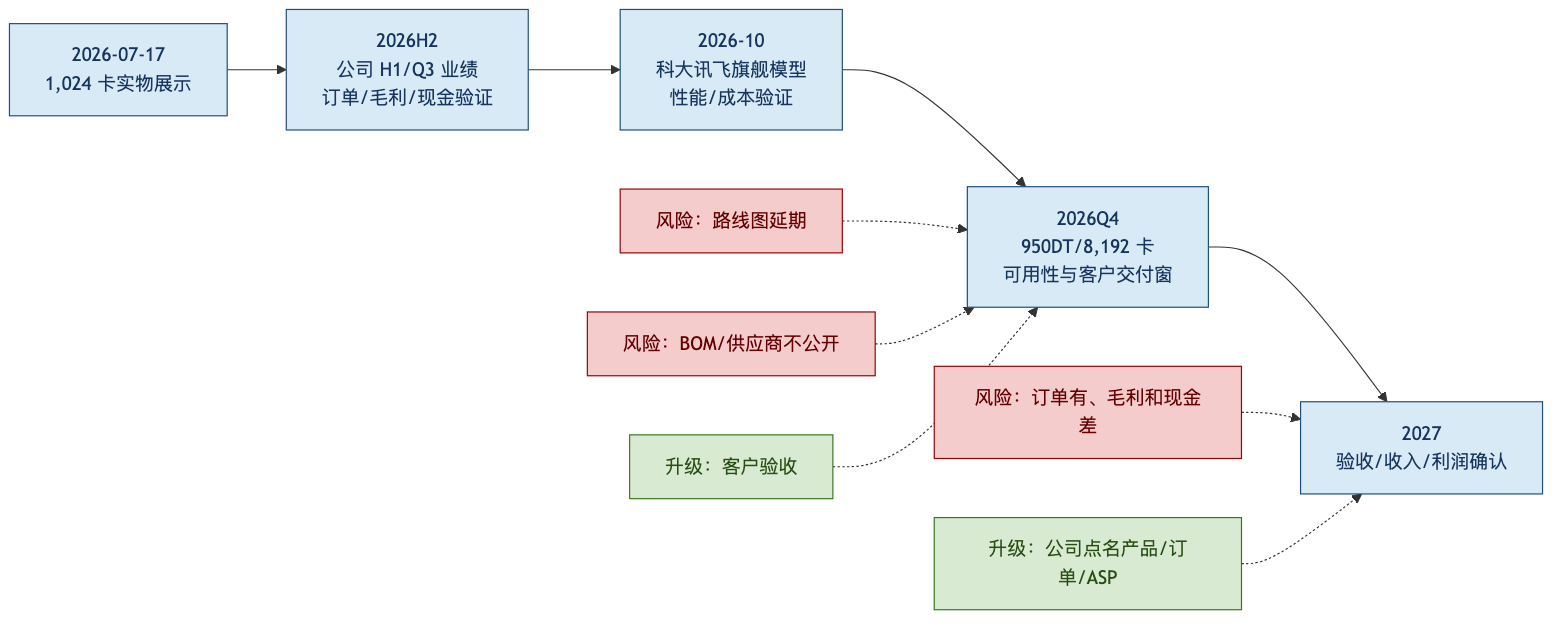
\includegraphics[width=\textwidth]{exhibits/catalyst_risk_timeline.png}
\caption{从实物展示到验收、收入与利润确认的催化/风险时间轴}
\sourcenote{华为路线图、科大讯飞年报与 AStock 风险矩阵。时间节点为验证窗口，不是自动收入确认日。}
\end{figure}

时间轴把技术事件与财务确认拆开：2026Q4 即使按时“可用”，仍需客户验收、公司产品/订单、ASP、收入与利润率证据；任何环节延期都会使盈利确认跨到 2027 年。相反，若客户验收与公司公告提前出现，当前零 Atlas 信用模型应立即更新。

2026Q3--Q4 监测 950DT 可用、客户、验收和生产负载；2026-12-31 前监测可复制商业部署与付款/收入；2027H1 监测稳定 8,192 卡客户系统；下一次技术披露监测 144GB HiZQ 本地 HBM 与 256TB 全局地址空间的关系；未来两个报告期监测供应商认证、订单、ASP、分部毛利、应收、存货和经营现金流；2026 年 10 月监测科大讯飞模型发布、成本性能和商业化。

十条发布红线包括：不得把实物 1,024 卡写成已交付 8,192 卡；不得把 256TB 写成 HBM；不得从传闻/投资者提问推导独家供应商；不得用前代装机、政策、运营商资本开支推导公司订单；不得无证据增加 Atlas EPS；不得无口径比较峰值 FLOPS；不得忽略管制与授权限制；不得在不知道用户组合的情况下给仓位；不得用上涨股价反驳证据缺口。

\section{结论改变条件}

风险评级下调需要多客户按期验收、稳定 8,192 卡生产负载、内存层级和量产良率得到解释、独立/客户负载验证 UnifiedBus 经济性、上市公司披露平台认证/订单/ASP/分部利润和现金流，同时估值没有进一步扩张。风险评级被确认则表现为：证据长期停留在展示与能力层，但价格继续定价独家供货、满规模交付和 Atlas 专属盈利。
